\documentclass{article}

\usepackage{xeCJK}
\setCJKmainfont{SimSun}

\usepackage{listings}
\lstset{breaklines,numbers=left}
\usepackage{hyperref}
\usepackage{pgf}
\usepackage{tikz}
\usetikzlibrary{arrows,shapes,snakes,automata,backgrounds,petri}

\title{FPGA Homework VII\thanks{%
        This homework report is source-opened on
        \href{https://github.com/Qinka/fgpa-homework}{GitHub:Qinka/fpga-homework}.
        Because one of my friend's Java homework, which is also opened on GitHub, was plagiarized by others, I just want declare the my, 李约瀚, copyleft(right) of the report of my homework.
        I, John Lee, is the only writer of this report.
    }}
\author{李约瀚 \\ 14130140331 \\ qinka@live.com \\ me@qinka.pro}

\begin{document}
    \maketitle
    \newpage
    \tableofcontents
    \newpage
    
    \section{Summary}
    \label{sec:summary}
    
    In this report of \textit{Homework VII}, there are practices in the text book, which is about a state machine and a counter,
    and design with instance, which is about the turnstile's instance with VHDL. In the practice of state machine, 
    the design has already done, and even the VHDL codes. So I combine them to simulate such a state machine on \textbf{ISim},
    and I got into trouble, when do post-route simulation, because of the ISE will not compiler the self-defined library, and
    resolution the record \textbf{\textit{MY\_RECORD}} to the basic types. After rewrite the rule of the compiling and 
    the test bench. The post-route simulation was done. In the practice of counter, I combine the codes of the other practices,
    and verified the behavior simulation and post-route simulation. For both of two practices, I test, or say find out,
    the highest frequencies of the circles. For the turnstile one, I design and instance one turnstile, and try to solve the
    competition of the putting and push signals. Then do the behavior simulation.
    
    
    \section{Pratice of State Machine}
    \label{sec:p:sm}
    
    In this part of the homework's report, the pratice is about the state machine.
    The state machine's changing graph, according to the text book, is the figure \ref{fig:sm:changing}.
    
    \begin{figure}[h!]
        \centering
        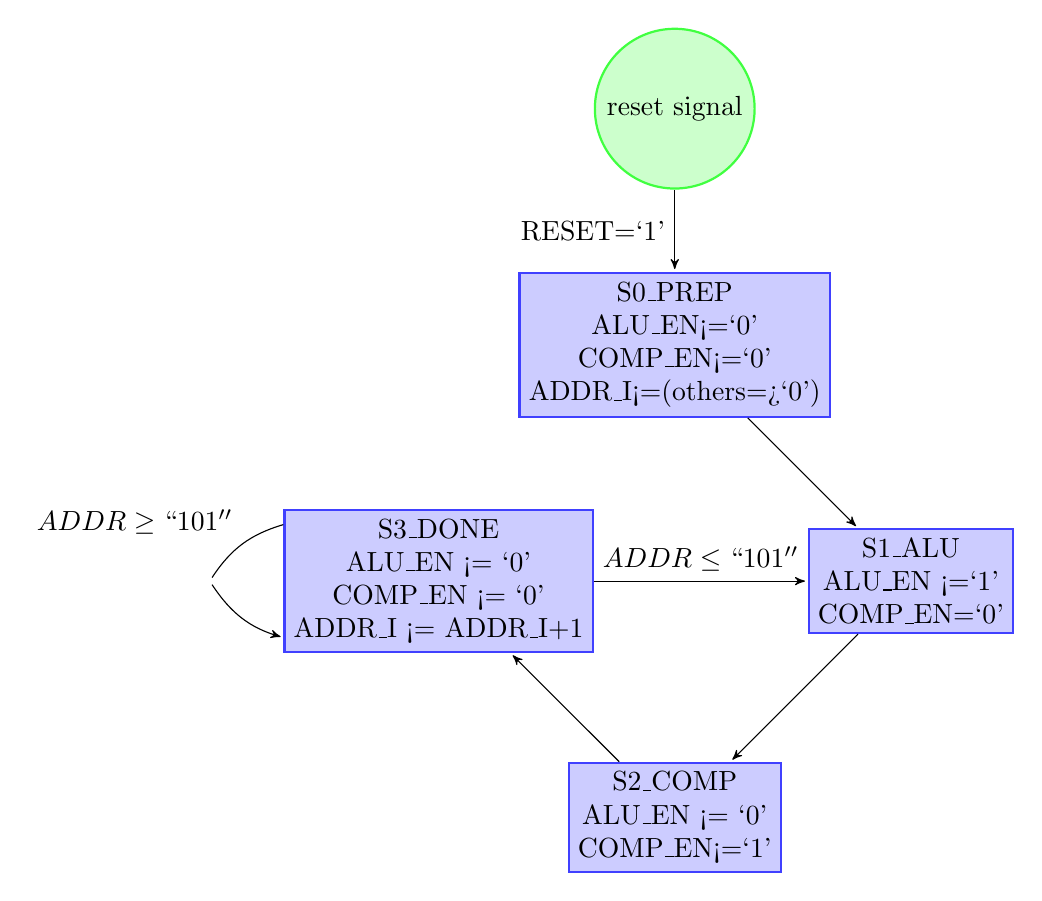
\begin{tikzpicture}[node distance=3cm,>=stealth',bend angle=20,auto]
        \tikzstyle{state}=[rectangle,thick,draw=blue!75,fill=blue!20,minimum size=8mm]
        \tikzstyle{signal}=[circle,thick,draw=green!75,fill=green!20,minimum size=6mm]
        \begin{scope}
        \node[signal](rst){reset signal};
        \node[state,align=center,below of=rst](s0){S0\_PREP \\ ALU\_EN<=`0'\\COMP\_EN<=`0'\\ADDR\_I<=(others=>`0')}
            edge [pre] node{RESET=`1'} (rst);
        \node[state,align=center,right of=s0,below of=s0](s1){S1\_ALU \\    ALU\_EN <=`1'\\COMP\_EN=`0'}
            edge [pre] (s0);
        \node[state,align=center,below of=s1,left of=s1](s2){S2\_COMP \\ ALU\_EN <= `0'\\COMP\_EN<=`1'}
            edge [pre] (s1);
        \node[state,align=center,left of=s0,below of=s0](s3){S3\_DONE \\ ALU\_EN <= `0' \\COMP\_EN <= `0' \\ ADDR\_I <= ADDR\_I+1}
            edge [pre] (s2)
            edge [post] node{$ADDR \leq ``101''$} (s1);
        \node[left of=s3](many){}
            edge [bend left] node{$ADDR \geq ``101''$} (s3)
            edge [post,bend right] (s3); 
        \end{scope}
        \end{tikzpicture}
        \caption{CNTRL\_FSM State Machine}
        \label{fig:sm:changing}
    \end{figure}
    
    \subsection{Instance}
    
    Then the according to the text, the codes in VHDL can be written.
    
    \begin{lstlisting}[language=VHDL,caption=CALC1 package]
library IEEE;
use IEEE.STD_LOGIC_1164.all;

package CALC1_PAK is

type MY_RECORD is record
A_IN : std_logic_vector ( 3 downto 0 ); 
B_IN : std_logic_vector ( 3 downto 0 );
OP_CODE : std_logic_vector ( 3 downto 0 );
C_IN : std_logic;
EXP_OUT : std_logic_vector ( 3 downto 0 );
end record MY_RECORD;

end package CALC1_PAK;
    \end{lstlisting}
    
    And the main part of the codes.
    \begin{lstlisting}[language=VHDL,caption=State Machine]
library IEEE;
use IEEE.STD_LOGIC_1164.all;
use IEEE.STD_LOGIC_ARITH.all;
use IEEE.STD_LOGIC_UNSIGNED.all;
use work.CALC1_PAK.all;

entity CNTRL_FSM1 is
    port ( DATA_FRAME : in  MY_RECORD;
           CLK        : in  std_logic;
           RESET      : in  std_logic;
           A_IN       : out std_logic_vector(3 downto 0);
           B_IN       : out std_logic_vector(3 downto 0);
           C_IN       : out std_logic;
           OP_CODE    : out std_logic_vector(3 downto 0);
           EXP        : out std_logic_vector(3 downto 0);
           ADDR       : out std_logic_vector ( 2 downto 0);
           COMP_EN    : out std_logic;
           MEM_EN     : out std_logic;
           ALU_EN     : out std_logic );
end entity CNTRL_FSM1;
architecture RTL of CNTRL_FSM1 is
    type CNTRL_STATE is ( S0_INIT, S1_FETCH, S2_ALU, S3_COMP, S4_DONE );
    signal CURR_STATE, NEXT_STATE : CNTRL_STATE;
    signal ADDR_I, ADDR_Q : std_logic_vector ( 2 downto 0 );
begin
    ADDR <= ADDR_Q;
    SYNC : process ( CLK, RESET )
    begin
        if ( RESET = '1' ) then
            CURR_STATE <= S0_INIT;
            ADDR_Q     <= ( others => '0' );
        elsif rising_edge (CLK) then
            CURR_STATE <= NEXT_STATE;
            ADDR_Q     <= ADDR_I;
        end if;
    end process SYNC;
    COMB : process ( CURR_STATE, DATA_FRAME, ADDR_Q )
    begin
        A_IN    <= DATA_FRAME.A_IN;
        B_IN    <= DATA_FRAME.B_IN;
        C_IN    <= DATA_FRAME.C_IN;
        OP_CODE <= DATA_FRAME.OP_CODE;
        EXP     <= DATA_FRAME.EXP_OUT;
        ADDR_I <= ADDR_Q;   
        case CURR_STATE is
            when S0_INIT =>
                MEM_EN  <= '0';
                ALU_EN  <= '0';
                COMP_EN <= '0';    
                NEXT_STATE <= S1_FETCH;
            when S1_FETCH =>
                MEM_EN  <= '1';
                ALU_EN  <= '0';
                COMP_EN <= '0';
                NEXT_STATE <= S2_ALU;
            when S2_ALU =>
                MEM_EN  <= '0';
                ALU_EN  <= '1';
                COMP_EN <= '0';
                NEXT_STATE <= S3_COMP;
            when S3_COMP =>
                MEM_EN  <= '0';
                ALU_EN  <= '0';
                COMP_EN <= '1';    
                NEXT_STATE <= S4_DONE;
            when S4_DONE =>
                if ADDR_Q >= "101" then
                    NEXT_STATE <= S4_DONE;
                else
                    NEXT_STATE <= S1_FETCH ;
                    ADDR_I <= ADDR_Q + 1;		         
                end if;	
                MEM_EN <= '0' ;
                ALU_EN <= '0';
                COMP_EN <= '0';
            when others =>
                NEXT_STATE <= S0_INIT;
                MEM_EN <= '0' ;
                ALU_EN <= '0';
                COMP_EN <= '0';				    
        end case;    
    end process COMB;
end RTL;
    \end{lstlisting}
    
    \subsection{Behavior Simulation}
    
    Next to be written is the test bench codes of the state machine.
    \begin{lstlisting}[language=VHDL,caption=Test Bench of State Machine]
library IEEE;
use IEEE.STD_LOGIC_1164.ALL;
use IEEE.STD_LOGIC_ARITH.ALL;
use IEEE.STD_LOGIC_UNSIGNED.ALL;
use work.CALC1_PAK.all;

ENTITY CNTRL_FSM_TB_vhd IS
END CNTRL_FSM_TB_vhd;
ARCHITECTURE TEST OF CNTRL_FSM_TB_vhd IS 
    COMPONENT CNTRL_FSM1
    PORT( DATA_FRAME : IN MY_RECORD;
        CLK : IN std_logic;
        RESET : IN std_logic;          
        A_IN : OUT std_logic_vector(3 downto 0);
        B_IN : OUT std_logic_vector(3 downto 0);
        C_IN : OUT std_logic;
        OP_CODE : OUT std_logic_vector(3 downto 0);
        EXP : OUT std_logic_vector(3 downto 0);
        MEM_EN : OUT std_logic;
        ALU_EN : OUT std_logic ;
        COMP_EN : OUT std_logic ;
        ADDR : OUT std_logic_vector(2 downto 0)
    );
    END COMPONENT;
    SIGNAL DATA_FRAME : MY_RECORD := ("0000", "0000","0000",'0',"0000");
    SIGNAL CLK :  std_logic := '0';
    SIGNAL RESET :  std_logic := '0';
    SIGNAL A_IN, B_IN :  std_logic_vector(3 downto 0);	 
    SIGNAL C_IN :  std_logic;
    SIGNAL OP_CODE :  std_logic_vector(3 downto 0);
    SIGNAL EXP :  std_logic_vector(3 downto 0);
    SIGNAL ALU_EN, MEM_EN, COMP_EN  :  std_logic;
    SIGNAL ADDR :  std_logic_vector(2 downto 0);
BEGIN
    uut: CNTRL_FSM1 PORT MAP(
    DATA_FRAME => DATA_FRAME,
    CLK => CLK,
    RESET => RESET,
    A_IN => A_IN,
    B_IN => B_IN,
    C_IN => C_IN,
    OP_CODE => OP_CODE,
    EXP => EXP,
    ALU_EN => ALU_EN, MEM_EN => MEM_EN, COMP_EN => COMP_EN ,
    ADDR => ADDR	);
    CLK <= not CLK after 20 ns;
    RESET <= '1' after 10 ns, '0' after 25 ns;    
    tb : PROCESS
    BEGIN
        DATA_FRAME <= ("1000", "0100","0000",'0',"0000");		 
        wait for 100 ns;
        DATA_FRAME <= ("1000", "0100","0101",'0',"0000");		 
        wait for 100 ns;
        DATA_FRAME <= ("1000", "0100","0100",'0',"0000");
        wait;
    END PROCESS;
END TEST;
    \end{lstlisting}
    
    Then the behavior level simulation's results are figure \ref{fig:homework7-1} and figure \ref{fig:homework7-2}.
    
\begin{figure}[h!]
\centering
\includegraphics[width=1\linewidth]{homework7-1}
\caption{The Result (1) of The Behavior Level Simulation}
\label{fig:homework7-1}
\end{figure}
\begin{figure}
\centering
\includegraphics[width=1\linewidth]{homework7-2}
\caption{The Result(2) of The Behavior Level Simulation}
\label{fig:homework7-2}
\end{figure}

    \subsection{Post-route Simulation}

    Then there goes the post-route level simulation of the state machine.
    There is a little but in ISE. Our library will not be able to compile.
    And the port of the one VHD, used to post-route simulation, is changed.
    
    
    First of all\footnote{We need be failed on post-route simulation, so that the files, we might need, can be generated.},
    the ``implement design'' is needed to be done.
    The VHD\footnote{E.g. netgen/par/CNTRL\_FSM1\_timesim.vhd} for port-route simulation can be found in the directory,
    named ``netgen/par'', under the project's work path.
    
    
    \begin{lstlisting}[language=VHDL,caption=One Version of The Entity for Post-route Simulation]
entity CNTRL_FSM1 is
    port (
        DATA_FRAME_C_IN : in STD_LOGIC := 'X'; 
        CLK : in STD_LOGIC := 'X'; 
        RESET : in STD_LOGIC := 'X'; 
        C_IN : out STD_LOGIC; 
        COMP_EN : out STD_LOGIC; 
        MEM_EN : out STD_LOGIC; 
        ALU_EN : out STD_LOGIC; 
        DATA_FRAME_A_IN : in STD_LOGIC_VECTOR ( 3 downto 0 ); 
        DATA_FRAME_B_IN : in STD_LOGIC_VECTOR ( 3 downto 0 ); 
        DATA_FRAME_OP_CODE : in STD_LOGIC_VECTOR ( 3 downto 0 ); 
        DATA_FRAME_EXP_OUT : in STD_LOGIC_VECTOR ( 3 downto 0 ); 
        A_IN : out STD_LOGIC_VECTOR ( 3 downto 0 ); 
        B_IN : out STD_LOGIC_VECTOR ( 3 downto 0 ); 
        OP_CODE : out STD_LOGIC_VECTOR ( 3 downto 0 ); 
        EXP : out STD_LOGIC_VECTOR ( 3 downto 0 ); 
        ADDR : out STD_LOGIC_VECTOR ( 2 downto 0 ) 
        );
end CNTRL_FSM1;
    \end{lstlisting}
    
    And then we need rewrite the port instance and the port binding, according to the new definition in the file for
    post-route simulation. The following is the new test bench.
    
    \begin{lstlisting}[language=VHDL,caption=Test Bench for Post-route Simulation]
library IEEE;
use IEEE.STD_LOGIC_1164.ALL;
use IEEE.STD_LOGIC_ARITH.ALL;
use IEEE.STD_LOGIC_UNSIGNED.ALL;
library work;
use work.CALC1_PAK.all;

ENTITY CF_TB_PR_vhd IS
END CF_TB_PR_vhd;
ARCHITECTURE TEST OF CF_TB_PR_vhd IS 
    COMPONENT CNTRL_FSM1
        port ( DATA_FRAME_C_IN : in STD_LOGIC := 'X'; 
            CLK : in STD_LOGIC := 'X';
            RESET : in STD_LOGIC := 'X'; 
            C_IN : out STD_LOGIC; 
            COMP_EN : out STD_LOGIC;
            MEM_EN : out STD_LOGIC; 
            ALU_EN : out STD_LOGIC; 
            DATA_FRAME_A_IN : in STD_LOGIC_VECTOR ( 3 downto 0 ); 
            DATA_FRAME_B_IN : in STD_LOGIC_VECTOR ( 3 downto 0 ); 
            DATA_FRAME_OP_CODE : in STD_LOGIC_VECTOR ( 3 downto 0 ); 
            DATA_FRAME_EXP_OUT : in STD_LOGIC_VECTOR ( 3 downto 0 ); 
            A_IN : out STD_LOGIC_VECTOR ( 3 downto 0 ); 
            B_IN : out STD_LOGIC_VECTOR ( 3 downto 0 ); 
            OP_CODE : out STD_LOGIC_VECTOR ( 3 downto 0 ); 
            EXP : out STD_LOGIC_VECTOR ( 3 downto 0 ); 
            ADDR : out STD_LOGIC_VECTOR ( 2 downto 0 ) 
        );
    END COMPONENT;
    SIGNAL DATA_FRAME : MY_RECORD := ("0000", "0000","0000",'0',"0000");
    SIGNAL CLK :  std_logic := '0';
    SIGNAL RESET :  std_logic := '0';
    SIGNAL A_IN, B_IN :  std_logic_vector(3 downto 0);	 
    SIGNAL C_IN :  std_logic;
    SIGNAL OP_CODE :  std_logic_vector(3 downto 0);
    SIGNAL EXP :  std_logic_vector(3 downto 0);
    SIGNAL ALU_EN, MEM_EN, COMP_EN  :  std_logic;
    SIGNAL ADDR :  std_logic_vector(2 downto 0);
BEGIN 
    uut: CNTRL_FSM1 PORT MAP(
        DATA_FRAME_C_IN => DATA_FRAME.C_IN,
        DATA_FRAME_A_IN => DATA_FRAME.A_IN,
        DATA_FRAME_B_IN => DATA_FRAME.B_IN,
        DATA_FRAME_OP_CODE => DATA_FRAME.OP_CODE,
        DATA_FRAME_EXP_OUT => DATA_FRAME.EXP_OUT,
        CLK => CLK,
        RESET => RESET,
        A_IN => A_IN,
        B_IN => B_IN,
        C_IN => C_IN,
        OP_CODE => OP_CODE,
        EXP => EXP,
        ALU_EN => ALU_EN, MEM_EN => MEM_EN, COMP_EN => COMP_EN ,
        ADDR => ADDR	);    
    CLK <= not CLK after 20 ns;
    RESET <= '1' after 10 ns, '0' after 25 ns;    
    tb : PROCESS
    BEGIN
        DATA_FRAME <= ("1000", "0100","0000",'0',"0000");		 
        wait for 100 ns;
        DATA_FRAME <= ("1000", "0100","0101",'0',"0000");		 
        wait for 100 ns;
        DATA_FRAME <= ("1000", "0100","0100",'0',"0000");
        wait; -- will wait forever
    END PROCESS;
END TEST;
    \end{lstlisting}    
    
    Then rewrite the project file, by coping a new one and modifying. Such a file might be like the following:
    
    \begin{lstlisting}
vhdl work "netgen/par/CNTRL_FSM1_timesim.vhd"
vhdl work "CNTRL_FSM_TB.vhd"
    \end{lstlisting}
    
    That basically means there is a vhdl source need to be added to ``work'' library, whose name is ``*.vhdl''.
    We need change them, to compile our new test bench file, self-defined library, and generated post-route simulation file.
    
    And it might be:
    
\begin{lstlisting}
vhdl work "CALC1_PAK.vhd"
vhdl work "netgen/par/CNTRL_FSM1_timesim.vhd"
vhdl work "CF_TB_PR.vhd"
\end{lstlisting}

    Finally, the new project file need be to ``point'' as custom project file in the properties of the 
    ``Simulation Post-Place \& Route Model''.
    
    And the result of the post-route simulation will be there: figure \ref{fig:homework7-3}, and figure \ref{fig:homework7-4}.
    
\begin{figure}
\centering
\includegraphics[width=1\linewidth]{homework7-3}
\caption{Post-route Simulation Result (1)}
\label{fig:homework7-3}
\end{figure}

\begin{figure}
\centering
\includegraphics[width=1\linewidth]{homework7-4}
\caption{Post-route Simulation Result (2)}
\label{fig:homework7-4}
\end{figure}

    \subsection{Analyze}

    According to the figure \ref{fig:homework7-4}, the delay about 6 ns. For each over-turn of the clock's signal,
    the feedback turn out after the stimulus reached, and the delay must be lower than the period.
    So the maximum of the clock's frequency is about 166.66MHz, but that is unstable. 
    I think 100MHz will be the maximum, and 50MHz is the one stable.
    The device utilization summary is the table \ref{tab:sm:dus}
    
    \begin{table}[h!]
        \centering
        \begin{tabular}{|c|c|c|c|}
            \hline Slice Logic Utilization & Used & Available & Utilization \\ 
            \hline Number of Slice Registers & 8 & 18,224 & 1\%
            \\ 
            \hline Number of Slice LUTs & 5 & 9,112 & 1\% \\ 
            \hline Number of occupied Slices & 2 & 2,278 & 1\% \\ 
            \hline Number of MUXCYs used & 0 & 4,556 & 0\%
            \\ 
            \hline Number of bonded IOBs & 42 & 232 & 18\% \\ 
            \hline 
        \end{tabular}
        \caption{Device Utilization Summary for State Machine}
        \label{tab:sm:dus}
    \end{table}
    
    \section{Practice of Counter}
    
    In this part of the report, we will create a counter, which is combined with the memory,
    comparer, ALU and state machine.
    Those devices' source are the ones in the previous practices, and I do nearly any change.
    
    \subsection{Instance}
    
    Only the top level ``SIMPLE\_CALC.VHD'' will give out, because othes source is not written at this time.
    
    The top level ``link'' the state machine, ALU, memory, and comparer\footnote{Both of RTL and behavior}, 
    as well as, define a new device -- ``SIMPLE\_CALC''.
    
    The ``program'' hardcoded in the memory is the following.    
    \begin{table}[h!]
        \centering
        \begin{tabular}{|c|c|c|c|c|}
            \hline A\_IN & B\_IN & C\_IN & OP\_CODE & EXP\_OUT \\ 
            \hline 1000 & 0010 & 0 & 0001 & 1010 \\ 
            \hline 0100 & 0010 & 0 & 0001 & 0110 \\ 
            \hline 0010 & 0010 & 0 & 0001 & 0100 \\ 
            \hline 0001 & 0010 & 0 & 0001 & 1111 \\ 
            \hline 0011 & 0010 & 0 & 0001 & 0101 \\ 
            \hline 0111 & 0010 & 0 & 0001 & 1001 \\ 
            \hline 
        \end{tabular} 
        \caption{The Test Program in Memory}
    \end{table}
    And the $4^{th}$ ``EXP\_OUT'' is error, and that is used to test the comparer.
    
    The following is the code of the top level.
    
    \begin{lstlisting}[language=VHDL,caption=Top-level of SIMPLE\_CALC]
library IEEE;
use IEEE.STD_LOGIC_1164.ALL;
use IEEE.STD_LOGIC_ARITH.ALL;
use IEEE.STD_LOGIC_UNSIGNED.ALL;
use work.CALC1_PAK.all;

entity SIMPLE_CALC is
    generic ( SYNTH : boolean := false );
    port ( CLK_IN : in std_logic;
        RESET: in std_logic;				   
        RESULT_OUT : out std_logic);
end SIMPLE_CALC;
architecture STRUCTURAL of SIMPLE_CALC is
    COMPONENT CNTRL_FSM1
        Port ( DATA_FRAME : in MY_RECORD;
            CLK : in std_logic;
            RESET : in std_logic ;
            A_IN : out std_logic_vector(3 downto 0);
            B_IN : out std_logic_vector(3 downto 0);
            C_IN : out std_logic;
            OP_CODE : out std_logic_vector(3 downto 0);
            EXP : out std_logic_vector(3 downto 0);
            ADDR : out std_logic_vector ( 2 downto 0);
            COMP_EN : out std_logic;
            ALU_EN : out std_logic;
            MEM_EN : out std_logic  
            );
    end component;
    COMPONENT ALU
        PORT(CLK : IN std_logic ;
            OP_CODE : IN std_logic_vector(3 downto 0);
            A : IN std_logic_vector(3 downto 0);
            B : IN std_logic_vector(3 downto 0);
            C_IN : IN std_logic;          
            Y : OUT std_logic_vector(3 downto 0);
            EN : in std_logic
            );
    END COMPONENT;
    COMPONENT MEM 
        Port ( CLK : std_logic ;
            EN : std_logic ;
            ADDR : in std_logic_vector(2 downto 0);
            DATA_FRAME : out MY_RECORD );
    end component;
    COMPONENT COMP
        PORT(CLK : in std_logic ;
            EXPECTED : IN std_logic_vector(3 downto 0);
            ALU_OUT : IN std_logic_vector(3 downto 0);          
            RESULT : OUT std_logic;
            EN : in std_logic
            );
    END COMPONENT;
    COMPONENT COMP_RTL
        PORT(CLK : in std_logic ;
            EXPECTED : IN std_logic_vector(3 downto 0);
            ALU_OUT : IN std_logic_vector(3 downto 0);          
            RESULT : OUT std_logic;
            EN : in std_logic
            );
    END COMPONENT;
    signal EXP_OUT_SIG : std_logic_vector ( 3 downto 0);
    signal A_IN_SIG : std_logic_vector ( 3 downto 0);
    signal B_IN_SIG :std_logic_vector ( 3 downto 0);
    signal OP_CODE_SIG :std_logic_vector ( 3 downto 0);
    signal CI_SIG : std_logic;
    signal ALU_EN_SIG : std_logic;
    signal COMP_EN_SIG : std_logic;
    signal MEM_EN_SIG : std_logic;
    signal ALU_OUT_SIG :std_logic_vector ( 3 downto 0);
    signal ADDR_SIG :std_logic_vector ( 2 downto 0);
    signal DATA_FRAME_SIG :MY_RECORD;
begin
    MEM_INST0: MEM PORT MAP(
        ADDR => ADDR_SIG,
        DATA_FRAME => DATA_FRAME_SIG,
        EN => MEM_EN_SIG,
        CLK => CLK_IN );
    ALU_INST0: ALU PORT MAP(
        OP_CODE => OP_CODE_SIG,
        A => A_IN_SIG,
        B => B_IN_SIG,
        C_IN => CI_SIG,
        Y => ALU_OUT_SIG,
        EN => ALU_EN_SIG,
        CLK => CLK_IN);    
    CNTRL_FSM_INST0: CNTRL_FSM1  PORT MAP(
        ADDR => ADDR_SIG,
        DATA_FRAME => DATA_FRAME_SIG,
        OP_CODE => OP_CODE_SIG,
        A_IN => A_IN_SIG,
        B_IN => B_IN_SIG,
        C_IN => CI_SIG,
        EXP => EXP_OUT_SIG,
        CLK => CLK_IN,
        RESET => RESET,
        ALU_EN => ALU_EN_SIG,
        COMP_EN => COMP_EN_SIG,
        MEM_EN => MEM_EN_SIG);
    GEN_SIM : if SYNTH = false generate 
    COMP_INST: component COMP port map(
        CLK => CLK_IN,
        EN => COMP_EN_SIG,
        EXPECTED => EXP_OUT_SIG,
        ALU_OUT => ALU_OUT_SIG,
        RESULT => RESULT_OUT);
    end generate GEN_SIM ;    
    GEN_SYNTH : if SYNTH = true generate 
    COMP_INST: component COMP_RTL port map(
        CLK => CLK_IN,
        EN => COMP_EN_SIG,
        EXPECTED => EXP_OUT_SIG,
        ALU_OUT => ALU_OUT_SIG,
        RESULT => RESULT_OUT);
    end generate GEN_SYNTH ;
end STRUCTURAL;
    \end{lstlisting}
    
    \subsection{Behavior Simulation}
    
    The thing to do is the behavior simulation.
    Firstly, the test bench is needed, and is the following one.
    
    \begin{lstlisting}[language=VHDL,caption=Test Bench of The Counter]
LIBRARY ieee;
USE ieee.std_logic_1164.ALL;
USE ieee.std_logic_unsigned.all;
USE ieee.numeric_std.ALL;

ENTITY SIMPLE_CALC_TB_vhd IS
END SIMPLE_CALC_TB_vhd;
ARCHITECTURE TEST OF SIMPLE_CALC_TB_vhd IS 
    COMPONENT simple_calc
        PORT(CLK_IN : IN std_logic;          
            RESET : in std_logic;
            RESULT_OUT : OUT std_logic
        ); 
    END COMPONENT;
    SIGNAL CLK_TB   :  std_logic := '0';
    SIGNAL RESET_TB :  std_logic := '0';
    SIGNAL RESULT 	:  std_logic;
BEGIN
    uut: simple_calc PORT MAP(
        CLK_IN => CLK_TB,
        RESET => RESET_TB,
        RESULT_OUT => RESULT
        ); 
    CLK_TB <= not CLK_TB after 10 ns;
    RESET_TB <= '1' after 5 ns, '0' after 10 ns, '1' after 700 ns, '0' after 725 ns;
END architecture TEST;
    \end{lstlisting}
    
    \begin{figure}[h!]
        \centering
        \includegraphics[width=1\linewidth]{homework7-5}
        \caption{Result of Counter's Behavior Simulation (1)}
        \label{fig:homework7-5}
    \end{figure}
    \begin{figure}[h!]
        \centering
        \includegraphics[width=1\linewidth]{homework7-6}
        \caption{Result of Counter's Behavior Simulation (2)}
        \label{fig:homework7-6}
    \end{figure}
    
    After synthesized, I select behavior simulation in the ISE, and run ISim. The figure \ref{fig:homework7-5}
    and figure \ref{fig:homework7-6} are the results of the simulation. And in the both of the figures,
    there is a slot, where the result is not the `1'. That means, in our program, the deliberately set error is ``work''.
    
    \subsection{Post-route Simulation}
           

    For the post-route simulation of the counter, it is not as matter as that of state machine.
    There isn't any bug in the ISE, which is touched off.
    
    \begin{figure}
        \centering
        \includegraphics[width=1\linewidth]{homework7-7}
        \caption{Result of Counter's Post-route Simulation}
        \label{fig:homework7-7}
    \end{figure}
    \begin{figure}
        \centering
        \includegraphics[width=1\linewidth]{homework7-8}
        \caption{Result of Counter's Post-route Simulation}
        \label{fig:homework7-8}
    \end{figure}
        
    The test bench of the behavior simulation is available, with no need for writing a new one.
    Figure \ref{fig:homework7-7} and figure \ref{fig:homework7-8} are the post-route simulation
    result, with the delay.

    \subsection{Analyze}
    
    According to the some kinds of summaries, there are some analyses.
    According to the \textit{Auto-Generated Design Constranints} analysis' summary,
    the minimum period is 1.897ns, and that means the maximum frequency is 527.148MHz.
    Meanwhile the minimum input required time, before the clock signal, is 2.462ns, and 
    the maximum output delay after clock is 7.344ns, that means the maximum frequency of the clock
    is about 136.166MHz. However, the 100MHz might be maximum stable one, and 50MHz might be the best frequency for work.

    \begin{table}[h!]
        \centering
        \begin{tabular}{|c|c|c|c|}
            \hline Slice Logic Utilization & Used & Available & Utilization\\
            \hline Number of Slice Registers & 20 & 18,224 & 1\% \\ 
            \hline Number used as Flip Flops & 20 &  &  \\ 
            \hline Number of Slice LUTs & 12 & 9,112 & 1\% \\ 
            \hline Number of LUT Flip Flop pairs used & 15 &  &  \\ 
            \hline Number of bonded IOBs & 3 & 232 & 1\% \\ 
            \hline 
        \end{tabular} 
        \caption{Device Utilization Summary}
        \label{tab:c:dus}
    \end{table}
    
    The table \ref{tab:c:dus} is the device utilization summary.
    
    
    
    
    \section{Practice of Turnstile}
    \label{sec:turnstile}
    
    \subsection{Design}
    \label{sec:turnstile:design}
    
    The turnstile is a small gate that spins around and only lets one person at a time go through an entrance%
    \footnote{Page 1901, \textit{Longman Dictionary of Contemporary English(New Edition)}, \textcopyright Pearson Education Limited, 1978,2009}.
    There are just two main actions: put in the coin and push the gate. So the state of turnstile should has two: locked
    and unlocked.
    Then the general state transition table will be table \ref{tab:tuenstile:state_transition}.
    \begin{table}[h!]
        \centering
        \begin{tabular}{|c|c|c|c|}
            \hline Current State & Stimulation & Next State & Note \\ 
            \hline Unlocked & putting coin & Unlocked & refuse the coin \\ 
            \hline Unlocked & pushing & Locked &  \\ 
            \hline Locked & putting coin & Unlocked &  \\ 
            \hline Locked & pushing & Locked & refuse the ``pushing'' \\ 
            \hline 
        \end{tabular}
        \caption{State Transition Table of Turnstile}
        \label{tab:tuenstile:state_transition}
    \end{table}
    
    With such a table, the graph of the state transition can be draw, and it is figure.
    
    \begin{figure}[h!]
        \centering
        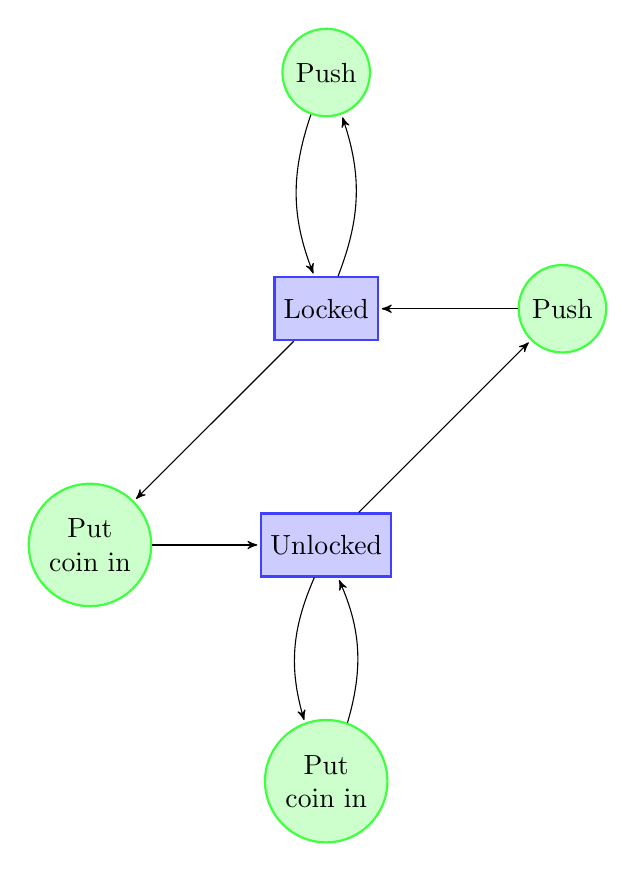
\begin{tikzpicture}[node distance=3cm,>=stealth',bend angle=20,auto]
            \tikzstyle{state}=[rectangle,thick,draw=blue!75,fill=blue!20,minimum size=8mm]
            \tikzstyle{signal}=[circle,thick,draw=green!75,fill=green!20,minimum size=6mm]
            \begin{scope}
            \node[state](locked){Locked};
            \node[state,below of=locked](unlocked){Unlocked};
            \node[signal,above of=locked](lockpush){Push}
                edge [pre,bend left] (locked)
                edge [post,bend right] (locked);
            \node[signal,below of=unlocked,align=center](unlockcoin){Put\\coin in}
                edge [pre,bend left] (unlocked)
                edge [post,bend right] (unlocked);
            \node[signal,below of=locked,left of=locked,align=center](lockcoin){Put\\coin in}
                edge [pre] (locked)
                edge [post] (unlocked);
            \node[signal,above of=unlocked,right of=unlocked](unlockpush){Push}
                edge [post] (locked)
                edge [pre] (unlocked);
            \end{scope}        
        \end{tikzpicture}
        \caption{State Transition Graph of Turnstile}
    \end{figure}
    
    So the input of turnstile has two signals: ``push'' and ``put coin in'', and the output signal is the state of turnstile.
    
    \subsection{Instance}
    \label{sec:turnstile:instance}
    
    To prevent the competition of signals, which are about pushing, and putting coin in, we need a clock signal to be arbiter. When clock signal rising,
    the signal for putting coin in is valid, and when clock signal falling,
    the signal for pushing is valid.
    The two input signals and the clock signal are combined to represent the state.
    And the following are the codes.
    
    \begin{lstlisting}[language=VHDL,caption=Turnstile Codes]
library IEEE;
use IEEE.STD_LOGIC_1164.ALL;

entity turnstile is
    Port ( coin : in  STD_LOGIC;
        push : in  STD_LOGIC;
        clock : in STD_LOGIC; -- 1 coin; 0 push
        lock : out  STD_LOGIC := '0'); -- 1 unlock
end turnstile;

architecture Behavioral of turnstile is
    signal state : STD_LOGIC_VECTOR(2 downto 0);
    signal lock_reg : STD_LOGIC := '0';
begin
    state <= coin & push & clock;
    lock <= lock_reg;
    process (clock)
    begin
        case state is
            when "111" => 
                lock_reg <= '1';
            when "110" =>
                lock_reg <= '0';
            when "101" =>
                lock_reg <= '1';
            when "010" =>
                lock_reg <= '0';
            when others =>
                lock_reg <= lock_reg;
        end case;
    end process;
end Behavioral;
    \end{lstlisting}
    
    \subsection{Behavior Simulation}
    
    So the turnstile will be test with these situations:
    \begin{itemize}
        \item no input signal
        \item put coin in when locked
        \item put coin in when unlocked
        \item push gate when locked
        \item push gate when unlocked
        \item put coin in and push gate at the same time when locked
        \item put coin in and push gate at the same time when unlocked
    \end{itemize}
    
    The test bench is the following codes.
    
    \begin{lstlisting}[language=VHDL,caption=Turnstile Test Bench]
LIBRARY ieee;
USE ieee.std_logic_1164.ALL;

ENTITY turnstile_tb IS
END turnstile_tb;
ARCHITECTURE behavior OF turnstile_tb IS 
    COMPONENT turnstile
        PORT(
            coin : IN  std_logic;
            push : IN  std_logic;
            clock : IN  std_logic;
            lock : OUT  std_logic
            );
    END COMPONENT;
    signal coin : std_logic := '0';
    signal push : std_logic := '0';
    signal clock : std_logic := '0';
    signal lock : std_logic;
    constant clock_period : time := 10 ns;
BEGIN
    uut: turnstile PORT MAP (
        coin => coin,
        push => push,
        clock => clock,
        lock => lock
        );
    clock_process :process
    begin
        clock <= '0';
        wait for clock_period/2;
        clock <= '1';
        wait for clock_period/2;
    end process;
    stim_proc: process
    begin
        wait for clock_period*9;
        push <= '1';
        wait for clock_period*2;
        push <= '0';
        coin <= '1';
        wait for clock_period*2;
        coin <= '0';
        wait for clock_period*2;
        coin <= '1';
        wait for clock_period*2;
        coin <= '0';
        push <= '1';
        wait for clock_period*2;
        coin <= '1';
        wait for clock_period*2;
        coin <= '0';
        push <= '0';
    end process;
END;

    \end{lstlisting}
   
   \begin{figure}[h]
        \centering
        \includegraphics[width=1\linewidth]{homework7-9}
        \caption{Result of Turnstile's Behavior Simulation (1)}
        \label{fig:homework7-9}
    \end{figure}

    \begin{figure}[h]
        \centering
        \includegraphics[width=1\linewidth]{homework7-10}
        \caption{Result of Turnstile's Behavior Simulation}
        \label{fig:homework7-10}
    \end{figure}
    
    The results of simulation are figure \ref{fig:homework7-9} and figure \ref{fig:homework7-10}.
    
    \subsection{Analyze}
    
    Such a turnstile has a disadvantage. Clock's frequency is sensitive.
    When clock frequency is high and two input signal arrived, the state of the
    turnstile will also turn over in a high frequency, but when clock's frequency
    is lower, and the responding will be lower too.
            
\end{document}